\section{Background and Related Work}
\label{sec:related}
%In this section, we present the motivations for this work by introducing the background and prior related studies.

\subsection{Machine Learning Project Licensing}
% 现在 ML 的license的现状,包括数据的license问题
Typically, a ML project is constructed with data, software and models, which are usually governed by different licensing frameworks.
To profile current ML licensing, we summary licensing details for ML projects with over 1,000 likes available in Huggingface model repository (See Appendix~\ref{apdx:A}).
Due to a lack of license management in development, we have to manually collect the license information from Huggingface, GitHub, related websites and publications.

\textbf{Data Licensing in ML}.
Based on our profile, half of ML projects claim their data is licensed in a mixture manner.
Additionally, 25\% of projects use a single dataset with a standard data license like Creative Commons (CC).
The data source of remaining projects (25\%) is unknown.
Obviously, legal compliance cannot be guaranteed when using data from unknown sources. 
However, there is also potential risk associated with using datasets under a mixture of licenses or a single license based on follow reasons:

First, the mixture of data sources may involve content under copyleft, non-public, and non-commercial licenses. 
We investigated the sources of mixture and found that only one dataset, the Pile~\cite{gao2020the}, explicitly removed non-permissive content.
Common sources of risk include Wikipedia, arXiv, PubMed and Common Crawl~\cite{henderson2023foundation} (See Table.~\ref{tab:works} for more examples).
For instance, sharing derivatives based on non-public licensed content raises suspicion of a license violation, and integrating copyleft content also poses a risk of license incompatibility conflicts.
Furthermore, some content sources like IMDb explicitly prohibit data mining in their \textit{Conditions of Use}\footnote{"You may not use data mining, robots, screen scraping, or similar data gathering and extraction tools on this site, ..."}.

Second, the single data license assigned by data collectors may be invalid.
In our profile, all datasets with a single license contain risky data sources.
Rajbahadur \textit{et al.}~\cite{rajbahadur2021can} investigated the sources of six public datasets and shown their inherent incompatibility for commercial use.
A real case is the copyright infringement lawsuit filed by Getty Images Inc., alleging that Stability AI Ltd. misused Getty Images photos to train its StableDiffusion~\cite{rombach2022high} generative model (1:23-cv-00135).
However, the claimed license of training dataset~\cite{schuhmann2022laion} used for StableDiffusion is CC-BY-4.0, which is a permissive license allowing for commercial use.
This highlights that ML data licensing is currently irregular and has become a significant factor in legal non-compliance.
Although Benjamin et al.~\cite{benjamin2019towards} have proposed the Montreal Data License (MDL) to foster fair use of data in AI activities, unfortunately, none of the ML projects adopted this license as shown in our profile.

\textbf{Software Licensing in ML.}
Distinct from OSS projects, only 50\% of ML projects release their code with standard OSS licenses.
About one-third of ML projects do not declare the code license (but have a model license), which is much higher than in OSS projects~\cite{cui2023empirical}.
Other projects switch to using AI model or custom licenses to insert additional disclaimers and restrictions related to AI activities, thereby increasing the diversity of licenses in this context.
However, given that ML, especially Neural Networks (NNs), is still in its emerging stages, the license dependency chain is shorter compared to OSS projects~\cite{buchkova2022dasea}, and most of them use the latest versions of OSS licenses like Apache-2.0 and MIT.

% 加一个license的统计数据?

\textbf{Model Licensing in ML.}
In contrast to software licensing, all ML projects have declared their model licenses.
The most popular license is Open Responsible AI License (OpenRAIL)~\cite{contractor2022behavioral}, which is a permissive license but includes copyleft-style use-based restrictions governing the use of the model and its derivatives.
There are 35\% of projects that insist on using unmodified OSS licenses for model licensing, even though these licensing language incurs conceptual ambiguities in the ML context.
An interesting finding is that, despite their training data being suspected to contain non-public content, the models are declared as free and open work~\cite{henderson2023foundation}.

%\vspace{-0mm}
\begin{tcolorbox}
\textbf{Summary}.
ML project licenseing exhibit the following characteristics:
1) Ambiguous, unaccredited and over-permissive license declarations;
2) Emerging RAIL options for model licensing;
3) Unique license dependency structures in ML-specific components reusing.
There is a need for new methods to assess ML license compliance.
\end{tcolorbox}


% 分歧:自定义license,使用 content license (LayoutLMv3, i2vgen)

\subsection{OSS License Assessment}
License analysis for OSS projects has been extensively researched, but it's relatively unexplored in ML context.
The research scope and problems of OSS and ML license analysis can be classified into three tiers as shown in Figure~\ref{fig:pyramid}.
%, which can be divide into code level and software level.
%The code level mainly focus on the compliance of a single file or lines of code.
For instance, German \textit{et al.}~\cite{german2010sentence} proposed a sentence-based matching tool to identify the license of code.
Building on this work, Wu \textit{et al.}~\cite{wu2017analysis} further studied inconsistent changes among code clones through provenance analysis.
In addition to license identification~\cite{jaeger2017fossology}, Vendome et al.~\cite{vendome2017machine} proposed a ML-based clustering method to detect license exceptions.
These studies mainly deal with copyright issues at the code lines level, located in bottom tier of Figure~\ref{fig:pyramid}, which can be mapped to similar ML problems: finding the provenance of data sources~\cite{rajbahadur2021can} or modules~\cite{chen2022copy}.
However, these OSS tools perform software composition analysis through pattern matching or file scanning~\cite{ombredanne2020free}, which are not suitable to datasets and models that typically lack clear provenance and textual licenses.

Shifting the focus to the middle tier, there are some studies that explore license compatibility and violations in software packages~\cite{mathur2012empirical, wu2015method}. 
Kapitsaki et al.~\cite{kapitsaki2017automating} used Software Package Data Exchange (SPDX) files to detect conflicts in license compatibility (e.g., GPL-2.0 to GPL-3.0).
Cui \textit{et al.}~\cite{cui2023empirical} directly extracted terms from license texts using Natural Language Processing (NLP) to analyze license conflicts in OSS projects.
\textbf{However, OSS license analysis works exhibit clear limitations when extended to ML projects.}
First, they lack support for dataset and model licenses. For example, RAILs and CCs are not listed in the SPDX. 
Second, the mixed use of licenses in current ML projects makes it challenging to interpret license conditions across different frameworks.
Last, these works only consider code replications and links in their analysis, whereas ML reuse involves a nested and iterative workflow with a more complex dependency structure (e.g., fine-tuning, embedding).

Distinct with previous studies, the research scope of our work is located in top and middle tiers.
we propose a practical tool ModelGo to assess potential license violations and non-granting righs errors in ML context.
We hope that ModelGo can assist developers in comprehending their obligations and risks when reusing ML components with multiple licenses~\cite{almeida2017software}, providing insights for constructing compliant ML systems.


\begin{figure}[t]
    \centering
    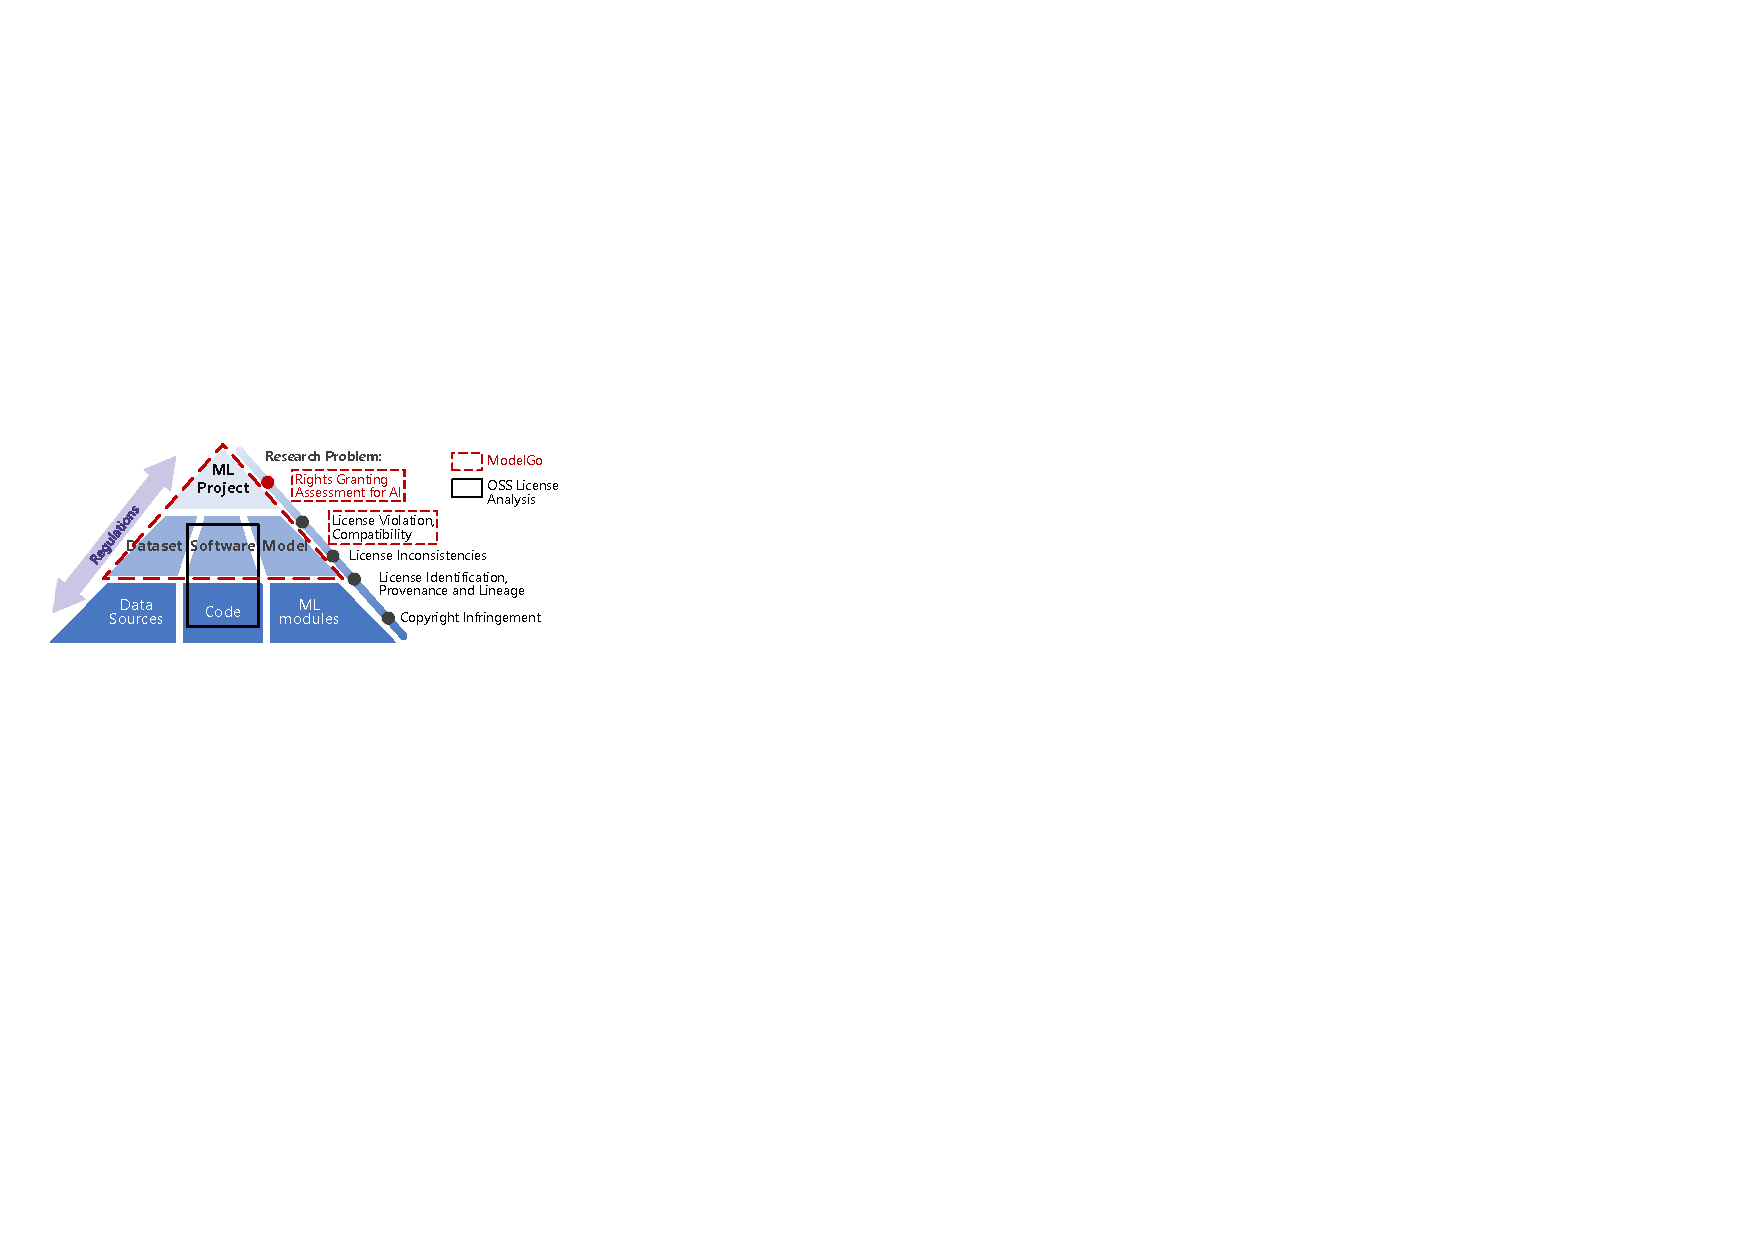
\includegraphics[width=\linewidth]{fig/pyramid.pdf}
    \caption{Research scope and problems of ModelGo compare with traditional OSS license analysis.}
    \Description{}
    \label{fig:pyramid}
\end{figure}

%\subsection{Machine Learning IP Protection}
% 检测是否transfer knowledge,与本工作不冲突


\begin{comment}
    There is no consensus on whether the use of copyright works as input to train an AI system is an exercise of an exclusive right.
    There remains significant legal uncertainty about whether copyright applies to AI training, which means it may not always be clear whether a CC license applies.
    The larger model was trained on 256 cloud TPU v3 cores. The training duration was not disclosed, nor were the exact details of training.
    
    Open source software license compliance~\cite{ombredanne2020free}
    
    The open source definition~\cite{perens1999open}
    
    AFL~\cite{rosen2005open}
    
    Wudao2.0 1.75T MoE
    [FASTMOE: A FAST MIXTURE-OF-EXPERT TRAINING SYSTEM]
    [GLM-130B: AN OPEN BILINGUAL PRE-TRAINED MODEL]
    
    Objectives and challenges associated with analyzing dataset license compliance?
    Getty Images (US), Inc. v. Stability AI, Inc. (1:23-cv-00135)
    Andersen et al v. Stability AI Ltd. et al (3:23-cv-00201)
    We are not aware of any copyright restrictions of the material
    
    C4, Pile Common Crawl
    crowdsourced
    
    COCO (CC-BY 4.0), CIFAR10 -> Flickr
    Unsplash License \textit{Custom}: Compiling photos from Unsplash to replicate a similar or competing service. https://unsplash.com/license
    Pixabay License: Data mining, extraction, scraping and the use of programs or robots for automatic data collection and/or extraction of digital data on the Services and/or the content available therein is strictly prohibited for all purposes, including without limitation for machine learning purposes.
    
    Google Street View (SVHN) https://about.google/brand-resource-center/products-and-services/geo-guidelines/
    
    %实际上,license analysis应该可分为四层,最底层是license 是否 compliance (或者叫做dataset provenance extraction, License identification),例如数据集的license是否可以覆盖每个sample,还有就是distribution的版本的license和official source的license不一致,第二层是license之间是否conflict,第三层是应用所需的rights是否具备,最顶层是应用场景是否符合法律法规(regulation)
    
    
    Software reuse is very simple from the legal point of view, if a company or an
    individual reuses software for which it has copyrights. However, things change dramatically
    if one wants to reuse software made by others, since software is protected
    by copyright and possibly by patents. Without explicit permission, no person other
    than the copyright holder is allowed to copy, distribute, or make derivative works
    from the original work.
\end{comment}

\begin{comment}
\begin{table*}[t]
    \caption{Summary of licensing details for machine learning projects with over 1K likes on Huggingface. }
    \footnotesize
    \label{tab:MLP}
    \begin{tabular}{|p{2.1cm}|p{1.6cm}|p{2cm}|p{2.75cm}|p{3cm}|p{1.7cm}|p{2cm}|}
        \hline
        \textbf{ML Project} & \textbf{Task} & \textbf{Data License} & \textbf{Software License} & \textbf{Model License} & \textbf{Dataset} & \textbf{Risk Resource} \\ \hline
        
        Stable Diffusion v1-5 & Text to Image & CC-BY-4.0 & CreativeML-OpenRAIL-M & CreativeML-OpenRAIL-M & LAION-5B & Common Crawl \\ \hline
        
        BLOOM & Text Generation & \textit{Mixture} & \textit{Unknown} & BigScience-BLOOM-RAIL-1.0 & \textit{Crowdsourced} & Common Crawl, \newline Wikipedia, etc. \\ \hline

        OrangeMixs & Text to Image & \textit{Mixture} & \textit{Unknown} & CreativeML-OpenRAIL-M & \textit{Crowdsourced} & Danbooru \\ \hline

        ControlNet & Text to Image &  \textit{Unknown} & Apache-2.0 & OpenRAIL & \textit{Unknown} & n/a \\ \hline

        Openjourney & Text to Image &  CC-BY-NC-4.0 & \textit{Unknown} & CreativeML-OpenRAIL-M & Midjourney Gen & Midjourney Gen \\ \hline

        ChatGLM-6B & Text Generation &  \textit{Mixture} & Apache-2.0 & \textit{Custom} & the Pile, Wudao, \newline \textit{Crowdsourced} & PubMed,  Wikipedia, \newline arXiv, GitHub, etc. \\ \hline

        Llama2 & Text Generation &  \textit{Unknown} & Llama2 Community License & Llama2 Community License & \textit{Unknown} & n/a \\ \hline

        StarCoder & Text Generation &  \textit{Mixture} & Apache-2.0 & BigCode-OpenRAIL-M & The Stack & none \\ \hline

        Falcon-40B & Text Generation & ODC-By & Apache-2.0 & Apache-2.0 & RefinedWeb & Wikipedia, Reddit, \newline StackOverflow, etc. \\ \hline

        Waifu Diffusion & Text to Image & \textit{Mixture} & \textit{Unknown} & CreativeML-OpenRAIL-M & \textit{Unknown} & n/a \\ \hline

        Dolly-v2-12B & Text Generation & CC-BY-SA-3.0\&4.0 & MIT & MIT & databricks-dolly\newline-15k, the Pile & PubMed,  Wikipedia, \newline arXiv, GitHub, etc. \\ \hline

        Dreamlike Photoreal & Text to Image & \textit{Unknown} & \textit{Unknown} & \textit{Modified} CreativeML-\newline OpenRAIL-M & \textit{Unknown} & n/a \\ \hline

        Counterfeit & Text to Image & \textit{Unknow} & \textit{Unknown} & CreativeML-OpenRAIL-M & \textit{Unknown} & n/a \\ \hline

        GPT-2 & Text Generation & \textit{Mixture} & \textit{Modified} MIT & \textit{Modified} MIT & \textit{Crowdsourced} & WordPress, GitHub, \newline wikiHow, IMDb, etc. \\ \hline

        GPT-J-6B & Text Generation & \textit{Mixture} & Apache-2.0 & Apache-2.0 & the Pile & PubMed,  Wikipedia, \newline arXiv, GitHub, etc. \\ \hline

        LLaMA-7B & Text Generation & \textit{Mixture} & \textit{Custom} & \textit{Custom} & \textit{Crowdsourced} & GitHub, arXiv, etc. \\ \hline

        BERT & Fill Mask & \textit{Mixture} & Apache-2.0 & Apache-2.0 & Book Corpus, \newline Wikipedia (en) & Wikipedia (en) \\ \hline

        Whisper & ASR & \textit{Unknown} & MIT & MIT & \textit{Unknown} & n/a \\ \hline

        MPT & Text Generation & \textit{Mixture} & Apache-2.0 & Apache-2.0 & \textit{Crowdsourced} & Common Crawl, \newline Wikipedia, etc. \\ \hline
    
    % <TOTAL>
    % Data License: All Permissive(2); Risk of Copyleft/Proprietary(11); Custom/Modified(0); Unknown(6);
    % Software License: Permissive(11); Risk of Copyleft/Proprietary(n/a); Custom/Modified(2); Unknown(6);
    % Model License: Permissive(15); Risk of Copyleft/Proprietary(n/a); Custom/Modified(4); Unknown(0);

    \end{tabular}
\end{table*}

\end{comment}